\documentclass[11pt,a4paper]{report}

\usepackage[T1]{fontenc}
\usepackage[utf8]{inputenc}
\usepackage{lmodern}
\usepackage{geometry}
\usepackage{microtype}
\usepackage{amsmath,amssymb}
\usepackage{graphicx}
\usepackage{booktabs}
\usepackage{tabularx}
\usepackage{array}
\usepackage{enumitem}
\usepackage{float}
\usepackage{caption}
\usepackage{xcolor}
\usepackage{fancyhdr}
\usepackage{hyperref}

\geometry{top=22mm,bottom=24mm,left=24mm,right=24mm,headheight=14pt}

\definecolor{reportnavy}{HTML}{0B2545}
\definecolor{reportblue}{HTML}{2563EB}
\definecolor{reportteal}{HTML}{0F766E}
\definecolor{reportorange}{HTML}{D97706}
\definecolor{reportpurple}{HTML}{7C3AED}
\definecolor{reportred}{HTML}{B91C1C}
\definecolor{reportgray}{HTML}{64748B}
\definecolor{reportlight}{HTML}{F4F7FA}

\hypersetup{
  colorlinks=true,
  linkcolor=reportblue,
  citecolor=reportteal,
  urlcolor=reportblue,
  pdftitle={Summer Research Internship Final Report},
  pdfauthor={Jeetraj and Prashit}
}

\captionsetup{
  font=small,
  labelfont={bf,color=reportnavy},
  labelsep=period,
  justification=centering
}

\setlength{\parindent}{0pt}
\setlength{\parskip}{0.62em}
\setlist[itemize]{leftmargin=1.5em,itemsep=0.25em,topsep=0.3em}
\setlist[enumerate]{leftmargin=1.7em,itemsep=0.25em,topsep=0.3em}
\renewcommand{\arraystretch}{1.18}
\setcounter{tocdepth}{0}
\setcounter{secnumdepth}{2}
\emergencystretch=2em

\pagestyle{fancy}
\fancyhf{}
\fancyhead[L]{\small SRI Final Report}
\fancyhead[R]{\small Adversarial Robustness and Attack Transfer}
\fancyfoot[C]{\thepage}
\renewcommand{\headrulewidth}{0.4pt}

\fancypagestyle{plain}{
  \fancyhf{}
  \fancyfoot[C]{\thepage}
  \renewcommand{\headrulewidth}{0pt}
}

\newcolumntype{Y}{>{\raggedright\arraybackslash}X}
\newcolumntype{C}[1]{>{\centering\arraybackslash}p{#1}}
\newcolumntype{L}[1]{>{\raggedright\arraybackslash}p{#1}}
\newcommand{\keybox}[1]{
  \begin{center}
  \fcolorbox{reportteal}{reportlight}{
    \parbox{0.91\textwidth}{#1}
  }
  \end{center}
}
\newcommand{\notebox}[1]{
  \begin{center}
  \fcolorbox{reportorange}{reportlight}{
    \parbox{0.91\textwidth}{#1}
  }
  \end{center}
}

\begin{document}

\begin{titlepage}
\thispagestyle{empty}
\centering

\vspace*{1.0cm}

{\Large\bfseries\color{reportnavy} SUMMER RESEARCH INTERNSHIP\par}
\vspace{0.25cm}
{\Large\bfseries\color{reportnavy} FINAL REPORT\par}

\vspace{1.3cm}

{\huge\bfseries Adversarial Robustness and\par}
\vspace{0.15cm}
{\huge\bfseries Cross-Victim Attack Transfer\par}

\vspace{0.55cm}

{\Large\color{reportteal}
DeepPoly Certification, Zero Knowledge Exploration,\par
and Reinforcement Learning\par}

\vspace{1.15cm}

\fcolorbox{black}{white}{
  \begin{minipage}{0.78\textwidth}
  \centering
  \vspace{0.25cm}
  \textbf{Mentor}\\[0.12cm]
  Prof. Manik Lal Das

  \vspace{0.45cm}

  \textbf{Students}\\[0.12cm]
  Jeetraj \hspace{0.25cm} Student ID: 202303017\\
  Prashit \hspace{0.25cm} Student ID: 202303049
  \vspace{0.25cm}
  \end{minipage}
}

\vfill

{\large DA-IICT, Gandhinagar\par}
\vspace{0.12cm}
{\large May to July 2026\par}

\end{titlepage}

\pagenumbering{roman}

\chapter*{Acknowledgement}
\addcontentsline{toc}{chapter}{Acknowledgement}

We sincerely thank Prof. Manik Lal Das for mentoring us during this Summer Research Internship. His guidance helped us move from an educational implementation of neural network verification to a broader study of privacy and adversarial attack transfer.

The internship gave us room to build, test, make mistakes, and improve our experimental method. We learned that a research result is useful even when the proposed method does not win, as long as the experiment is fair, reproducible, and reported without hiding negative evidence.

We also thank DA-IICT for providing the academic setting for this work.

\chapter*{Abstract}
\addcontentsline{toc}{chapter}{Abstract}

Small changes to an input can cause a neural network to change its prediction. This internship studied that problem from three connected viewpoints. We began with DeepPoly, a method that computes sound lower and upper bounds for neural network outputs. We implemented educational MNIST experiments and explored how certification can be included in training.

We then studied zero knowledge machine learning. The goal was to understand whether a robustness certificate could be checked while keeping a model or test data private. This part remained a research proposal. We did not implement a zero knowledge circuit or generate a proof.

The main experimental phase studied attack transfer with reinforcement learning. A recurrent PPO policy was trained on two source model families, frozen, and evaluated on a held-out victim family. The final CIFAR-10 study used three victim families, three seeds, a 25-query budget, and an \(L_\infty\) limit of \(8/255\). All victim-quality gates passed. However, frozen PPO reached only \(1.01\%\) to \(1.65\%\) mean attack success across target families and did not beat random search. Its action entropy stayed close to random. A score-guided greedy baseline achieved \(13.55\%\) to \(27.20\%\), although its proposal step was not identical to the PPO step.

The final outcome is a working research harness, a carefully audited negative result, and a clear set of next experiments. The study does not show that reinforcement learning can never transfer attacks. It shows that this PPO state, action, and reward design did not learn a useful transferable advantage under the tested conditions.

\tableofcontents
\clearpage
\pagenumbering{arabic}

\chapter{Introduction}

\section{The question that connected our work}

Neural networks can be accurate on normal inputs and still behave unexpectedly after a small change. A few pixels may be changed, a digit may be rotated, or a sound may be slightly perturbed. These changes can be hard for a person to notice but large enough to affect a model.

Our internship followed one central question:

\keybox{
\textbf{\color{reportnavy}How can we understand, verify, and test a neural network when its input changes slightly?}

DeepPoly studies this question from the defender's side. Zero knowledge proofs add a privacy question. Reinforcement learning studies it from the attacker's side.
}

The work did not start as one large system. It grew in stages. Each stage answered one question and exposed the next one.

\section{Main contributions}

The internship produced the following concrete outputs:

\begin{itemize}
  \item DeepPoly bound propagation and certification-aware training on MNIST;
  \item PGD, rotation, and speech attack explorations;
  \item a research map connecting neural verification with zero knowledge machine learning;
  \item a source-to-target attack framework with frozen and target-adaptation modes;
  \item a recurrent PPO and GroupDRO training pipeline for cross-victim transfer;
  \item random, score-bandit, and score-greedy controls under a shared query budget;
  \item a three-family, three-seed CIFAR-10 study run on an Apple M4;
  \item audit checks, figures, and reproducible result summaries.
\end{itemize}

\chapter{DeepPoly and Certified Robustness}

\section{Why normal accuracy is not enough}

Normal test accuracy measures predictions on a fixed dataset. It does not prove what happens to nearby inputs. Adversarial testing can find a failure, but a failed search does not prove that no failure exists.

Formal certification asks a stronger question. For an input \(x\) and radius \(\varepsilon\), define

\begin{equation}
\mathcal{B}_{\varepsilon}(x)
=
\left\{
x' \in [0,1]^d :
\lVert x' - x \rVert_{\infty} \leq \varepsilon
\right\}.
\end{equation}

The goal is to prove that every \(x'\) in this set has the same class as \(x\). This is harder than checking one adversarial example because the set contains infinitely many possible inputs.

\section{The DeepPoly idea}

DeepPoly propagates symbolic lower and upper bounds through the network \cite{singh2019deeppoly}. Affine layers can be handled with linear expressions. ReLU layers require a relaxation because the function changes form at zero.

For a neuron with pre-activation bounds \(l\) and \(u\), there are three cases:

\begin{enumerate}
  \item If \(l \geq 0\), the ReLU is always active and its output equals the input.
  \item If \(u \leq 0\), the ReLU is always inactive and its output is zero.
  \item If \(l < 0 < u\), the ReLU is uncertain and is enclosed by sound linear bounds.
\end{enumerate}

For an uncertain ReLU, a standard upper relaxation is

\begin{equation}
z
\leq
\frac{u}{u-l}(x-l).
\end{equation}

The abstraction may include values that no real input produces, so it can be conservative. However, it must not exclude any valid input in the perturbation set. That soundness is what makes a successful certificate meaningful.

\section{Certification rule}

Suppose class \(y\) is the predicted class. Let \(\ell_y\) be a lower bound for its output and \(u_j\) be an upper bound for every competing class. The sample is certified when

\begin{equation}
\ell_y > \max_{j \neq y} u_j.
\label{eq:certification}
\end{equation}

Equation~\ref{eq:certification} means that class \(y\) remains above every alternative for the complete abstract region.

\section{MNIST certification result}

The saved result compares a cross-entropy baseline with a model trained using a DeepPoly-based robustness term. The run evaluated 100 correctly classified MNIST samples.

\begin{figure}[H]
\centering
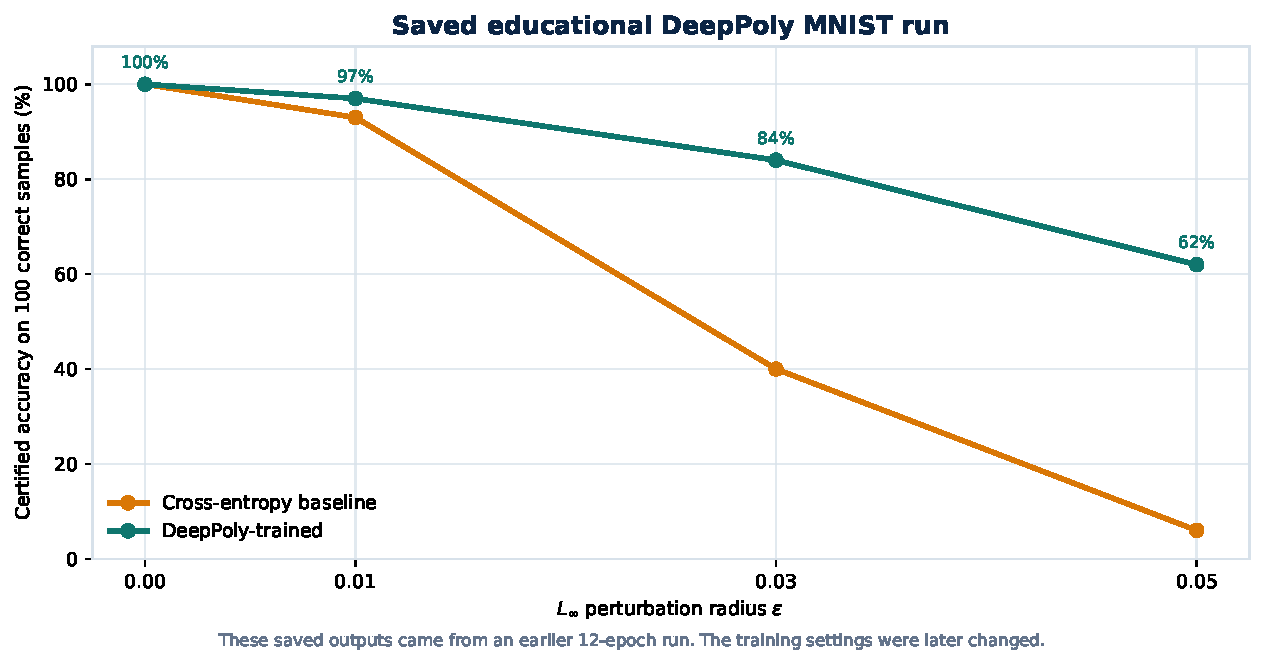
\includegraphics[width=0.88\textwidth]{figures/sri_deeppoly_certification.pdf}
\caption{Certified accuracy from the saved educational MNIST result.}
\label{fig:deeppoly-curve}
\end{figure}

At \(\varepsilon=0.05\), the saved output reported \(6\%\) certified accuracy for the baseline and \(62\%\) for the DeepPoly-trained model. The average certified margin changed from \(-5.8963\) to \(0.7822\). Clean test accuracy was similar: \(93.64\%\) for the baseline and \(94.12\%\) for the robust model.

\notebox{
\textbf{\color{reportnavy}Scope of this result.}
The plot comes from a saved 12-epoch educational run. The training settings were later revised, but a new result was not generated after that change. We therefore treat this as an early experiment rather than a tuned benchmark.
}

\section{Certification-aware training}

The training experiment combined normal classification loss with a bound-based penalty:

\begin{equation}
\mathcal{L}
=
\mathcal{L}_{\mathrm{CE}}
+
\lambda \mathcal{L}_{\mathrm{DP}}.
\end{equation}

Here, \(\mathcal{L}_{\mathrm{DP}}\) penalizes cases where a competing upper bound approaches or exceeds the true-class lower bound. The experiment also used an epsilon curriculum, where the training radius increases gradually.

This stage taught us an important distinction. Adversarial training searches for difficult examples and trains on them \cite{madry2018towards}. Certified training tries to improve a mathematical lower bound on robustness. They are related, but they do not make the same guarantee.

\chapter{Zero Knowledge Exploration}

\section{Why privacy entered the project}

Formal verification usually assumes that the verifier can access the network and the values used in the calculation. In a real deployment, the model owner may not want to reveal the weights. A data owner may also want to keep evaluation samples private.

Zero knowledge proofs study a different guarantee. A prover can convince a verifier that a computation was carried out correctly without revealing the private witness used in that computation.

\begin{table}[H]
\centering
\caption{DeepPoly and zero knowledge answer different questions.}
\begin{tabularx}{\textwidth}{p{0.22\textwidth} Y Y}
\toprule
 & \textbf{DeepPoly} & \textbf{Zero knowledge proof} \\
\midrule
Question &
Does the network keep its decision for every input in a defined perturbation set? &
Was a stated computation checked correctly without revealing the private witness? \\
\addlinespace
Typical private item &
Privacy is not the main purpose. &
Model weights, data, intermediate values, or other witness values. \\
\addlinespace
Main guarantee &
Sound robustness certificate for a defined threat model. &
Sound and private verification of a stated relation. \\
\bottomrule
\end{tabularx}
\end{table}

\section{Proposed certificate-checking workflow}

Our research notes proposed separating expensive bound generation from proof checking:

\begin{figure}[H]
\centering

\fcolorbox{reportblue}{reportlight}{
\parbox{0.72\textwidth}{
\centering
\textbf{Private model and selected evaluation data}\\
The prover owns the witness.
}}

\vspace{0.18cm}
\(\Downarrow\)
\vspace{0.18cm}

\fcolorbox{reportteal}{reportlight}{
\parbox{0.72\textwidth}{
\centering
\textbf{DeepPoly certificate generation}\\
Compute layer bounds and the final certified margin outside the proof.
}}

\vspace{0.18cm}
\(\Downarrow\)
\vspace{0.18cm}

\fcolorbox{reportpurple}{reportlight}{
\parbox{0.72\textwidth}{
\centering
\textbf{Proposed zero knowledge checker}\\
Check affine consistency, ReLU cases, ranges, and certified counts.
}}

\vspace{0.18cm}
\(\Downarrow\)
\vspace{0.18cm}

\fcolorbox{reportorange}{reportlight}{
\parbox{0.72\textwidth}{
\centering
\textbf{Public claim}\\
A stated number of samples satisfies the chosen robustness condition.
}}

\caption{Proposed private verification direction. This workflow was designed but not implemented.}
\label{fig:zk-flow}
\end{figure}

The checker would need constraints for affine layers, ReLU phase cases, fixed-point ranges, and the final class separation in Equation~\ref{eq:certification}. Recursive proof systems such as Nova \cite{kothapalli2022nova} and compact range proofs such as Bulletproofs \cite{bunz2018bulletproofs} were studied as possible supporting ideas.

Work such as zkCNN and ZEN shows that neural inference can be represented in zero knowledge proof systems \cite{liu2021zkcnn,feng2021zen}. Adding a complete robustness certificate is harder because bound propagation creates many intermediate values and comparison constraints.

\chapter{Reinforcement Learning for Attack Transfer}

\section{From verification to attack behavior}

DeepPoly asks whether a model is safe throughout a region. Our final experimental direction asked a complementary question: can an attacker learn behavior on some victims and reuse it against a different victim?

Transferability is useful in a realistic black-box setting. The target model may be expensive to query and its parameters may be hidden. An attack policy can train on available source models, then use only a small number of score queries on the target.

\section{Two modes of transfer}

The project supports two related modes. They should not be mixed when interpreting results.

\begin{table}[H]
\centering
\small
\caption{Frozen transfer and target adaptation.}
\begin{tabular}{@{}L{0.16\textwidth}L{0.36\textwidth}L{0.36\textwidth}@{}}
\toprule
 & \textbf{Frozen transfer} & \textbf{Target adaptation} \\
\midrule
Starting point &
Policy trained on source victims. &
Clone of a policy trained on source victims. \\
\midrule
Target-time learning &
No parameter update. Recurrent state may change within an episode. &
The clone may continue learning on a separate target adaptation subset. \\
\midrule
Main question &
Did the source policy learn behavior that transfers directly? &
Does source training provide a useful starting point for continued learning? \\
\midrule
Use in final study &
Yes. This is the evaluated scientific protocol. &
Implemented as framework support and smoke-tested, but not used for the final headline claim. \\
\bottomrule
\end{tabular}
\end{table}

For frozen transfer, the policy digest is recorded before and after target evaluation. Matching SHA-256 digests give direct evidence that policy parameters did not change.

\section{Victim families}

The study used three custom CIFAR-10 classifiers. Each victim was trained on 10,000 images for 12 epochs.

\begin{table}[H]
\centering
\small
\caption{Victim models used in the study.}
\begin{tabularx}{0.86\textwidth}{Y Y C{0.20\textwidth}}
\toprule
\textbf{Family} & \textbf{Architecture} & \textbf{Parameters} \\
\midrule
Classical CNN & Residual CNN & 2,777,674 \\
Modern CNN & Depthwise CNN & 1,223,738 \\
Transformer & Patch transformer & 347,722 \\
\bottomrule
\end{tabularx}
\end{table}

For each run, PPO trained against four source victims: two instances from each of two families. One model from the third family was kept for frozen evaluation. The three held-out settings were repeated with seeds 17, 29, and 41.

Each run used 1,000 policy-training images and 1,000 source-validation images. PPO scheduled 600 attack episodes, updated after every block of 25 episodes, and used four optimization passes per update. Final evaluation used 300 separate images.

\begin{figure}[H]
\centering
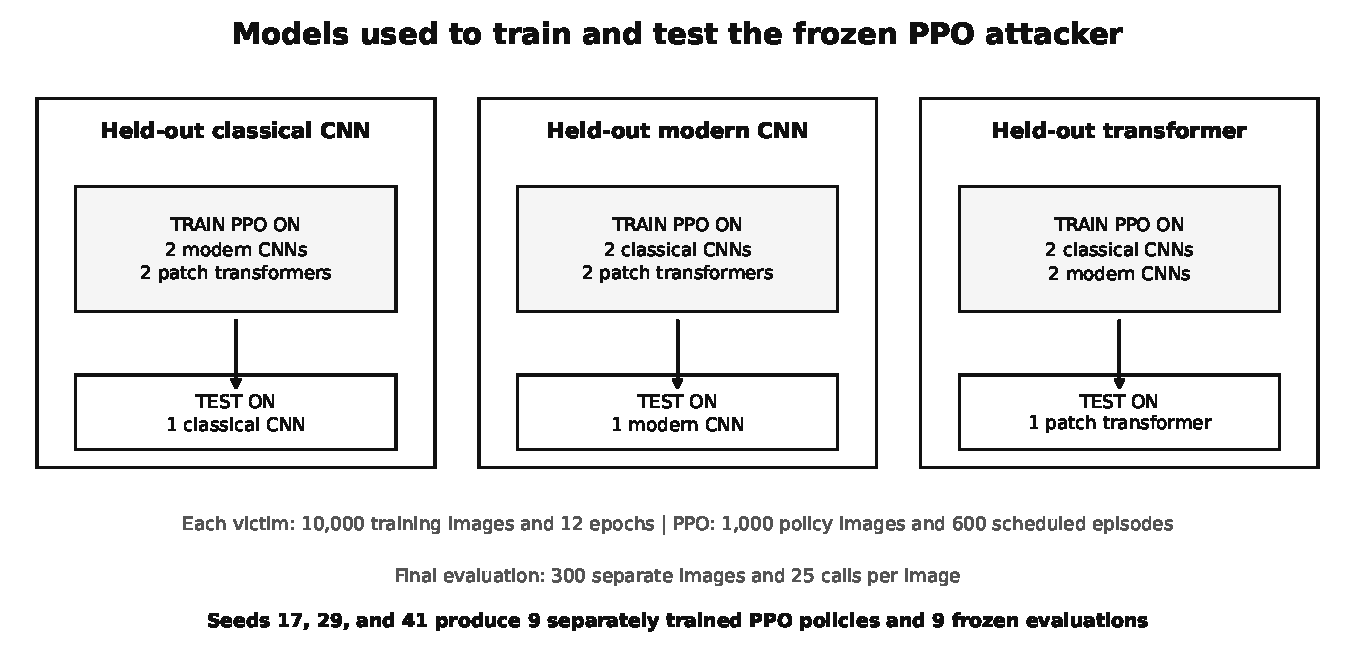
\includegraphics[width=\textwidth]{figures/sri_rl_train_test_design.pdf}
\caption{The exact source and target model arrangement used in the nine runs.}
\label{fig:rl-train-test}
\end{figure}

\section{RL agent structure}

The recurrent PPO policy \cite{schulman2017ppo} does not receive the raw image. It receives eight response features: correct-class rank, entropy, confidence change, confidence margin, remaining budget, previous action, previous reward, and attack progress.

The encoder maps these 8 values to 96 learned features. A 96-unit GRU carries memory across attack steps. The shared representation then splits into an actor and a critic. The actor produces 96 action logits, while the critic produces one value estimate.

\begin{figure}[H]
\centering
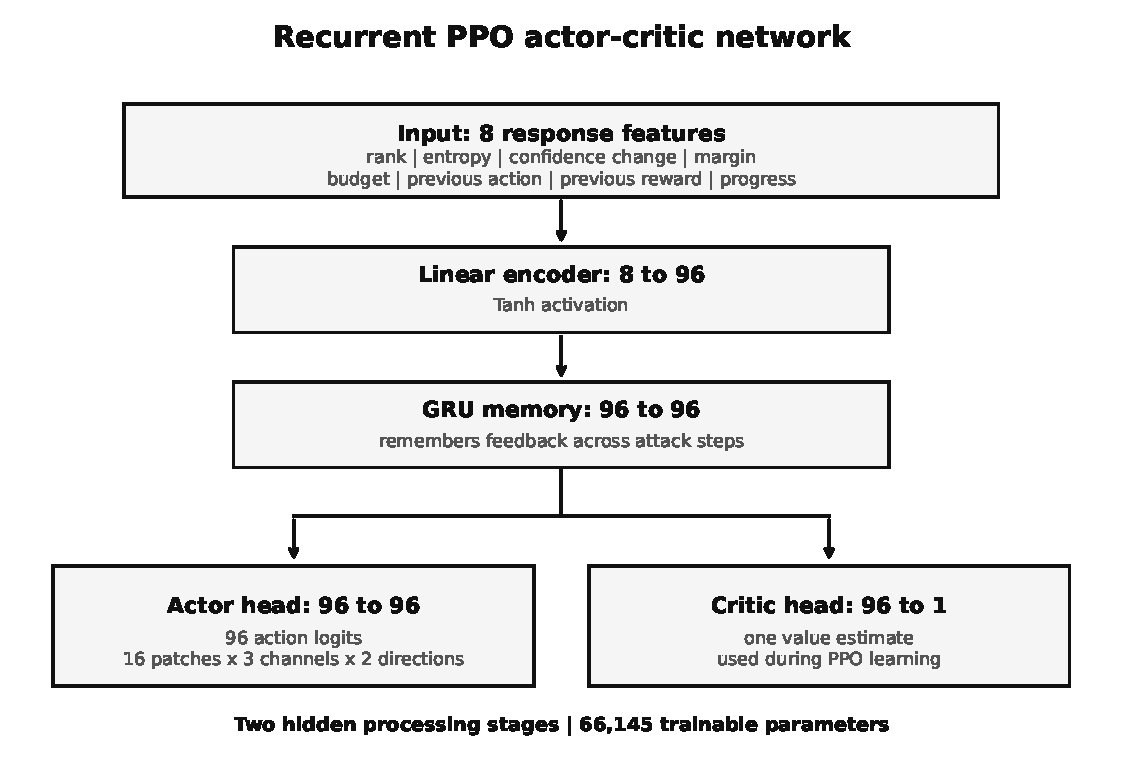
\includegraphics[width=0.91\textwidth]{figures/sri_rl_policy_architecture.pdf}
\caption{The recurrent PPO actor-critic network.}
\label{fig:rl-architecture}
\end{figure}

The complete policy has 66,145 trainable parameters. Its two hidden processing stages are the 96-unit encoder and the 96-unit GRU memory layer.

The image is divided into 16 patches. An action selects:

\begin{itemize}
  \item one of 16 patches;
  \item one of three color channels;
  \item a positive or negative direction.
\end{itemize}

The resulting discrete action space has

\begin{equation}
16 \times 3 \times 2 = 96
\end{equation}

actions. A PPO action proposes a step of \(2/255\). Every update is projected back into the allowed \(L_\infty\) region and clipped to valid image values:

\begin{equation}
x_{t+1}
=
\operatorname{clip}_{[0,1]}
\left(
\operatorname{clip}_{[x-\varepsilon,x+\varepsilon]}
\left(x_t+\delta(a_t)\right)
\right).
\end{equation}

\section{Reward and source-family balance}

Sparse success rewards gave too little learning signal in early experiments. The final version used the true-class margin

\begin{equation}
m_t
=
p_y(x_t)
-
\max_{j \neq y} p_j(x_t),
\end{equation}

and the dense reward

\begin{equation}
r_t
=
5(m_{t-1}-m_t)
+
2\,\mathbb{I}\!\left[f(x_t)\neq y\right]
-
0.01.
\label{eq:reward}
\end{equation}

The first term rewards margin reduction, the second rewards a successful misclassification, and the last term gives a small cost for using a step.

GroupDRO weighting was used to keep training from focusing only on the easiest source family \cite{sagawa2020groupdro}. Family losses and source-model calls were recorded for audit.

\chapter{Experimental Method}

\section{Threat model and query accounting}

The target evaluation used:

\begin{itemize}
  \item CIFAR-10 images \cite{krizhevsky2009cifar};
  \item an \(L_\infty\) limit of \(8/255\);
  \item 25 total target score calls, including initialization;
  \item only images correctly classified by the clean target model;
  \item the same eligible images for all compared methods;
  \item no target-family policy training or tuning in the frozen protocol.
\end{itemize}

\begin{figure}[H]
\centering
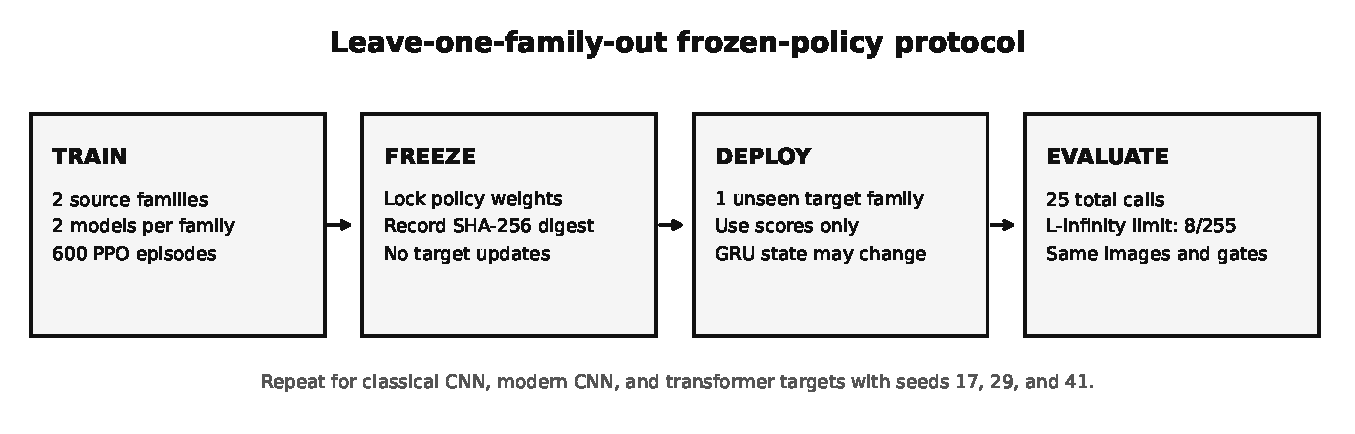
\includegraphics[width=\textwidth]{figures/sri_rl_protocol.pdf}
\caption{Training, freezing, deployment, and evaluation under the final protocol.}
\label{fig:rl-protocol}
\end{figure}

Every target call counts. Failed attempts are not removed. Lower-query measurements come from the same trajectory, so a method does not receive extra attempts at each query checkpoint.

\section{Controls}

Four methods were compared:

\begin{enumerate}
  \item \textbf{Stochastic PPO:} sample actions from the frozen learned policy.
  \item \textbf{Random:} sample uniformly from the same action catalog.
  \item \textbf{Score bandit:} use observed score changes to favor useful actions.
  \item \textbf{Score greedy:} test score-guided patch proposals and keep improvements.
\end{enumerate}

The score-greedy control shares the image set, final \(L_\infty\) limit, action catalog, and overall target-query budget. Its direct proposal magnitude is \(8/255\), while PPO uses \(2/255\) steps. It is therefore a strong reference for score-guided patch search, but not a perfectly matched comparison of identical update operators.

\section{Metrics}

The main metric is attack success rate:

\begin{equation}
\operatorname{ASR}(q)
=
\frac{
\text{successful attacks by query }q
}{
\text{clean-correct eligible target images}
}.
\end{equation}

We also measured the area under the ASR-by-query curve, confidence-margin reduction, action entropy, runtime, victim accuracy, and policy-digest stability.

The promotion rule was deliberately strict. It checked practical and statistical improvement over controls, acceptable action entropy for every seed, victim-quality gates, shared samples, exact budgets, and internal consistency. A missing or failed check caused the result to fail closed.

\section{Hardware and scale}

The full experiment ran locally on an Apple M4 with MPS acceleration. It completed in 6,864.9 seconds, or about 114.4 minutes.

\begin{table}[H]
\centering
\caption{Scale of the final CIFAR-10 study.}
\begin{tabularx}{0.88\textwidth}{Y C{0.28\textwidth}}
\toprule
\textbf{Item} & \textbf{Completed value} \\
\midrule
Held-out target families & 3 \\
Fresh seeds & 17, 29, 41 \\
Family and seed folds & 9 \\
Scheduled training episodes & 5,400 \\
Trainable sequences & 3,640 \\
Source-model calls & 91,800 \\
Clean-correct target image and run cases per method & 1,859 \\
Total target calls per image and method & 25 \\
Wall-clock time & 114.4 minutes \\
\bottomrule
\end{tabularx}
\end{table}

\chapter{Results}

\section{Victim-quality checks}

A transfer study is not useful if the victim models are too weak to classify clean data. Each family therefore had a minimum validation-accuracy gate. All nine folds passed.

\begin{figure}[H]
\centering
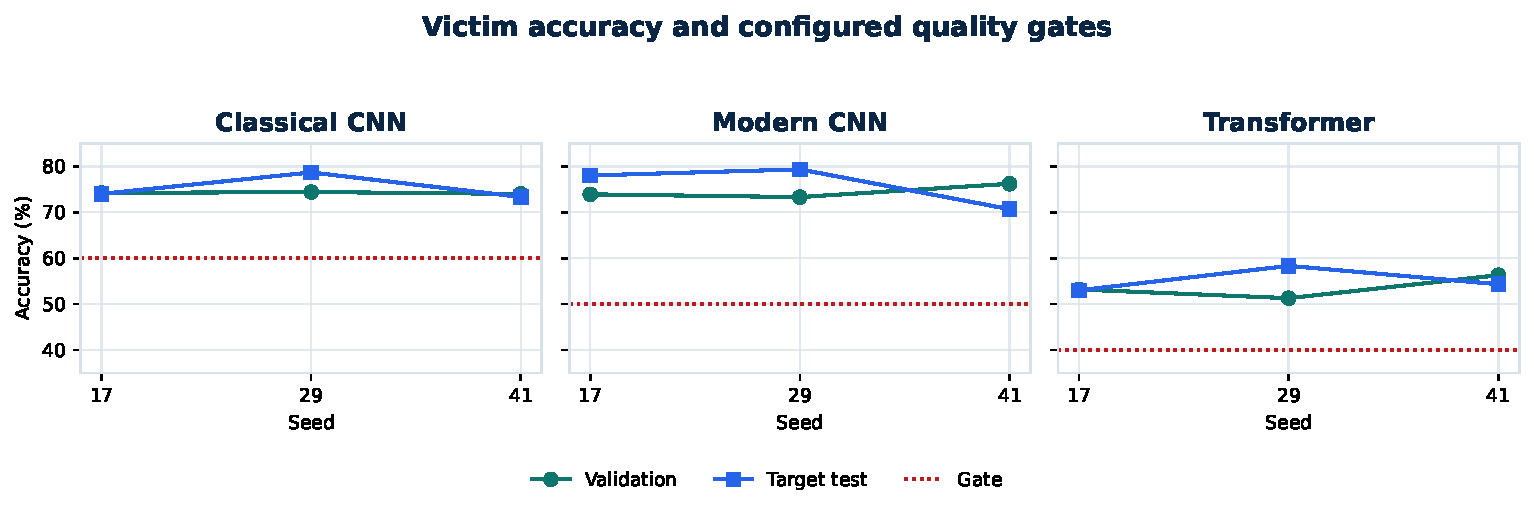
\includegraphics[width=\textwidth]{figures/sri_victim_accuracy.pdf}
\caption{Validation accuracy, target-test accuracy, and configured quality gates.}
\label{fig:victim-accuracy}
\end{figure}

\begin{table}[H]
\centering
\caption{Victim accuracy across the three study seeds.}
\begin{tabularx}{0.91\textwidth}{Y C{0.21\textwidth} C{0.16\textwidth} C{0.21\textwidth}}
\toprule
\textbf{Family} & \textbf{Validation range} & \textbf{Gate} & \textbf{Target-test range} \\
\midrule
Classical CNN & \(74.0\%\) to \(74.4\%\) & \(60\%\) & \(73.3\%\) to \(78.7\%\) \\
Modern CNN & \(73.3\%\) to \(76.2\%\) & \(50\%\) & \(70.7\%\) to \(79.3\%\) \\
Transformer & \(51.3\%\) to \(56.3\%\) & \(40\%\) & \(53.0\%\) to \(58.3\%\) \\
\bottomrule
\end{tabularx}
\end{table}

\section{Final attack success}

Figure~\ref{fig:final-asr} gives the across-seed mean ASR at 25 total target calls.

\begin{figure}[H]
\centering
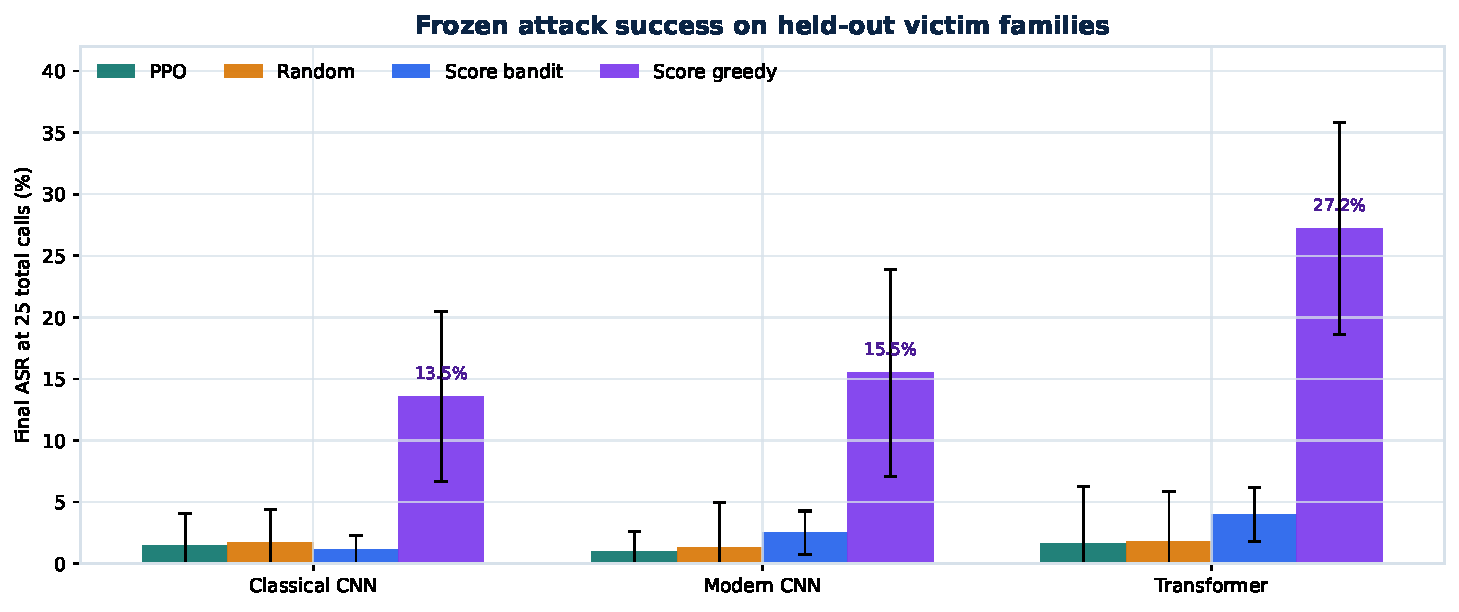
\includegraphics[width=\textwidth]{figures/sri_final_asr.pdf}
\caption{Mean final attack success rate across seeds 17, 29, and 41.}
\label{fig:final-asr}
\end{figure}

\begin{table}[H]
\centering
\caption{Mean final ASR on each held-out target family.}
\begin{tabularx}{\textwidth}{Y C{0.17\textwidth} C{0.17\textwidth} C{0.17\textwidth} C{0.17\textwidth}}
\toprule
\textbf{Held-out target} & \textbf{PPO} & \textbf{Random} & \textbf{Score bandit} & \textbf{Score greedy} \\
\midrule
Classical CNN & \(1.45\%\) & \(1.74\%\) & \(1.17\%\) & \(\mathbf{13.55\%}\) \\
Modern CNN & \(1.01\%\) & \(1.29\%\) & \(2.50\%\) & \(\mathbf{15.49\%}\) \\
Transformer & \(1.65\%\) & \(1.84\%\) & \(4.02\%\) & \(\mathbf{27.20\%}\) \\
\bottomrule
\end{tabularx}
\end{table}

PPO did not beat random on any family mean. It was slightly above the score-bandit mean on the classical target, but the full paired promotion rule still failed. Score greedy was much stronger on all three target families.

\section{Success across the query sequence}

Final ASR gives one endpoint. Figure~\ref{fig:query-curves} shows when successes appeared during the 25-call budget.

\begin{figure}[H]
\centering
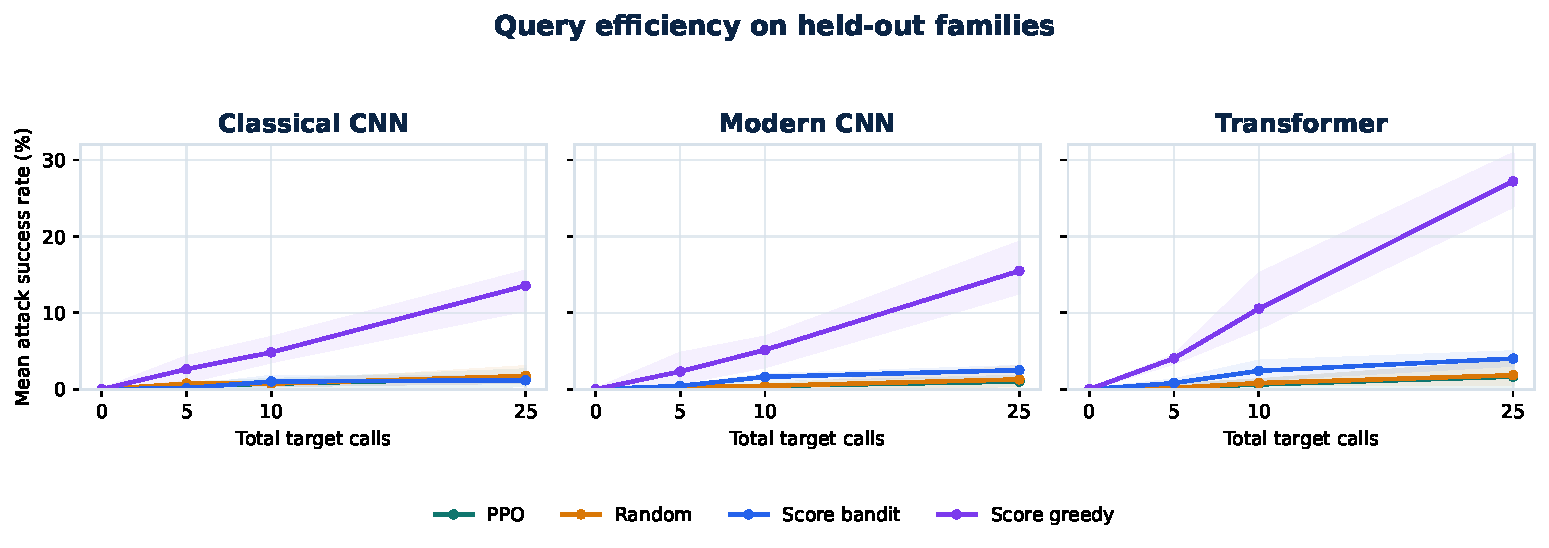
\includegraphics[width=\textwidth]{figures/sri_query_curves.pdf}
\caption{Across-seed ASR as the target-query budget is used.}
\label{fig:query-curves}
\end{figure}

The ASR-by-query area values were:

\begin{table}[H]
\centering
\caption{Area under the ASR-by-query curve. Higher is better.}
\begin{tabularx}{\textwidth}{Y C{0.17\textwidth} C{0.17\textwidth} C{0.17\textwidth} C{0.17\textwidth}}
\toprule
\textbf{Held-out target} & \textbf{PPO} & \textbf{Random} & \textbf{Score bandit} & \textbf{Score greedy} \\
\midrule
Classical CNN & 0.81 & 0.96 & 0.79 & 6.52 \\
Modern CNN & 0.53 & 0.62 & 1.48 & 7.17 \\
Transformer & 0.78 & 0.91 & 2.33 & 13.19 \\
\bottomrule
\end{tabularx}
\end{table}

The endpoint and query-curve results tell the same story. PPO did not gain an early or sustained advantage over random actions. Score-guided selection used the limited calls more effectively.

\section{What the action entropy revealed}

Normalized executed-action entropy measures how widely the policy spreads its selected actions. A value close to one indicates behavior close to a uniform action distribution.

\begin{figure}[H]
\centering
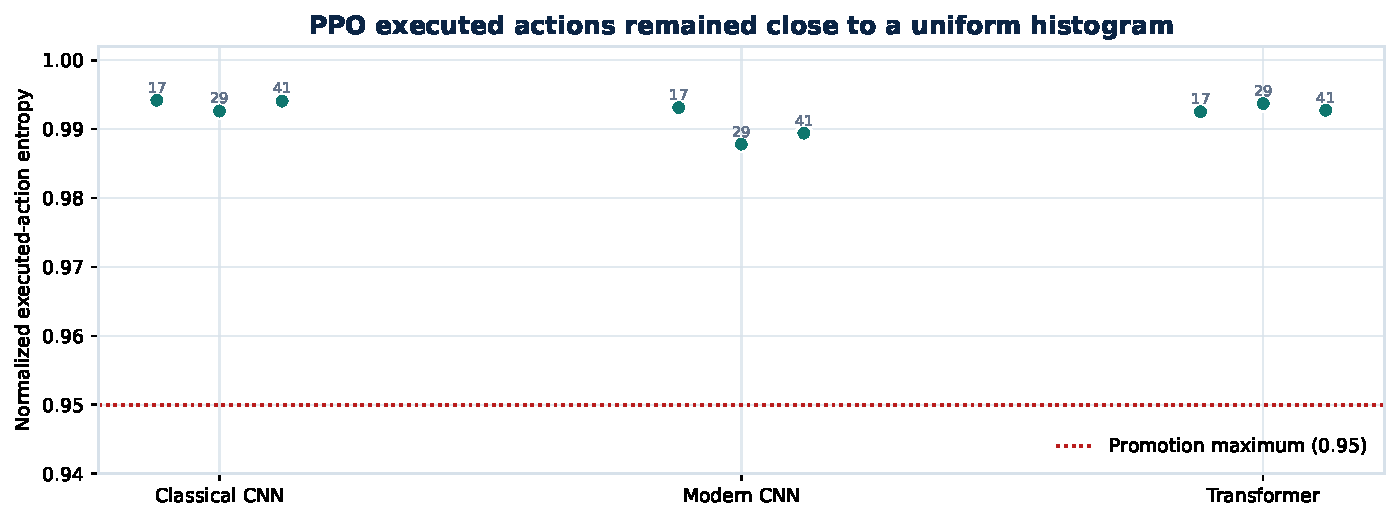
\includegraphics[width=0.88\textwidth]{figures/sri_action_entropy.pdf}
\caption{PPO executed-action entropy across target families. The promotion maximum was 0.95.}
\label{fig:entropy}
\end{figure}

PPO entropy stayed between 0.988 and 0.994. This exceeded the promotion maximum of 0.95 for every family. The learned policy had not developed a strong action preference, which agrees with its near-random ASR.

\section{Pilot and full-study comparison}

The first M4 pilot trained on a classical CNN and a modern CNN, then attacked a held-out patch transformer. It finished in 6 minutes 12 seconds. On 99 clean-correct images, stochastic PPO achieved \(5.1\%\) ASR and random achieved \(7.1\%\).

The pilot was useful because it verified the frozen-policy digest and the end-to-end MPS workflow. It also warned us not to claim an RL advantage from a single small run.

The full study improved the reward, victim fitting, source populations, controls, seeds, and audit rules. The stronger experiment reached the same broad conclusion: PPO did not establish a transfer advantage.

\section{Interpretation}

\keybox{
\textbf{\color{reportnavy}Main empirical conclusion.}
Under this CIFAR-10 setup, the recurrent GroupDRO PPO policy did not learn a useful frozen cross-victim advantage. All victim-quality gates passed, but the promotion gate failed for every held-out family.
}

This is a result about the tested design, not a universal result about reinforcement learning or attack transfer. The state was compact, the action catalog was coarse, the query budget was small, and only three custom victim families were used.

The score-greedy result is still informative. It shows that score-guided patch search can succeed in the same overall threat setting. It also suggests that the PPO policy did not extract enough value from score changes. Because score greedy used a larger direct proposal step, matched step-size ablations are needed before assigning the full gap to its search rule.

\section{Why the PPO success rate remained low}

The measurements point to a learning problem rather than a failed evaluation. All victim-quality gates passed, the policy stayed frozen during target testing, and score greedy found successful attacks on the same eligible images. The following evidence suggests likely causes, but only matched ablations can establish their separate effects.

\begin{table}[H]
\centering
\small
\caption{Measured evidence and likely effects on PPO learning.}
\begin{tabularx}{\textwidth}{L{0.31\textwidth}Y}
\toprule
\textbf{Measured evidence} & \textbf{What it suggests} \\
\midrule
Normalized PPO action entropy stayed between 0.988 and 0.994. &
The actor remained close to a uniform distribution over 96 actions. It did not learn a reliable preference for useful patches, channels, or directions. \\
\midrule
Only 64 of 3,640 trainable source episodes ended in success, a rate of \(1.76\%\). &
The terminal success bonus was rare. Most updates depended on small confidence-margin changes, which can be noisy and different across victims. \\
\midrule
Only 3,640 of 5,400 scheduled episodes produced PPO sequences, or \(67.4\%\). &
The other episodes were skipped because the selected source victim was already wrong on the clean image. The effective amount of policy training was therefore smaller than the schedule suggests. \\
\midrule
The observation contained eight global score features. &
It did not contain image content, a perturbation map, patch visit counts, or a full record of earlier patch effects. Different attack situations could therefore look similar to the policy. The GRU can remember received information, but it cannot recover information that was never observed. \\
\midrule
PPO used a fixed \(2/255\) step and had 24 attack calls after initialization. &
Reaching the \(8/255\) boundary in one direction required repeated compatible choices. A nearly uniform policy could spend much of the small query budget on weak or conflicting steps. \\
\midrule
PPO kept every proposed move, while score greedy kept only margin-reducing moves and proposed \(8/255\) changes. &
PPO could undo earlier progress. The stronger greedy result combines a score-guided search rule, rollback behavior, and a larger proposal, so the present experiment cannot assign the full gap to only one of these factors. \\
\midrule
Each run used four source victims from two families and one unseen target victim. &
This is enough to test the protocol, but it offers limited architectural diversity. Patch preferences learned on the source victims may not remain useful on the held-out family. \\
\bottomrule
\end{tabularx}
\end{table}

\chapter{Discussion and Next Work}

\section{Main lessons}

\begin{itemize}
  \item A successful attack shows that one failure exists. A sound certificate can prove robustness for every input inside a defined region.
  \item Frozen transfer and continued target learning are different experiments. The final result measures frozen transfer only.
  \item Controls are essential. PPO reached \(5.1\%\) in the pilot, but random search reached \(7.1\%\).
  \item Near-random action entropy showed that the policy had not learned a selective attack strategy.
\end{itemize}

\section{Limitations}

\begin{itemize}
  \item The DeepPoly result used 100 correctly classified MNIST samples from an early training configuration.
  \item The zero knowledge part remained a proposal and was not implemented.
  \item The RL study used CIFAR-10, three custom victim families, and three seeds.
  \item Each fold used one held-out target instance.
  \item PPO and score greedy used different proposal magnitudes.
  \item The result should not be generalized to larger pretrained models.
\end{itemize}

\section{How to improve RL attack success}

The next study should improve the learning signal, state representation, action design, and source diversity in a controlled order.

\begin{enumerate}
  \item \textbf{Match the proposal operator.}
  Give PPO, random, bandit, and greedy methods the same step sizes and the same accept-or-reject rule. Test \(2/255\), \(4/255\), and \(8/255\) as separate ablations. This will show whether the current gap comes mainly from action selection or from the stronger greedy proposal.

  \item \textbf{Keep the best candidate found so far.}
  After a query, retain a proposal only when it reduces the correct-class margin. A rejected proposal still consumes its query, but it does not damage the next state. The policy can also receive an explicit accepted-or-rejected feature.

  \item \textbf{Start from successful demonstrations.}
  Collect score-greedy trajectories on source victims and use behavior cloning to train the actor before PPO updates begin. PPO can then improve a selective starting policy instead of beginning from almost uniform actions.

  \item \textbf{Give the policy a richer observation.}
  Add patch visit counts, the signed score change caused by each recent action, current perturbation level per patch, recent accepted actions, and a short window of margin changes. A compact image or patch embedding can also be tested because it does not require access to target-model parameters.

  \item \textbf{Use hierarchical and multi-scale actions.}
  Let the policy choose a region, channel, direction, and step size in stages. Include coarse and fine patch grids. This can support large early moves, smaller refinements near the decision boundary, and clearer learning than one flat 96-action decision.

  \item \textbf{Increase the amount and quality of source training.}
  Build each episode from an image that the assigned source victim classifies correctly, so scheduled episodes are not lost. Begin with low-margin images, then move toward harder samples. Add more independently trained source instances and more architecture families after the policy beats random on source validation.

  \item \textbf{Tune exploration and reduce update variance.}
  Start with useful exploration and gradually reduce the entropy coefficient. Compare reward normalization per victim, generalized advantage estimation, learning-rate sweeps, and a larger success bonus. Monitor entropy, source ASR, validation ASR, critic error, and gradient norms so a uniform or collapsed policy is detected early.

  \item \textbf{Compare learning algorithms under the same operator.}
  If PPO remains uniform, compare it with a recurrent DQN and a score-aware contextual bandit. This checks whether the limitation comes from the PPO update or from the state and action design shared by all methods.

  \item \textbf{Evaluate target adaptation separately.}
  Clone the source policy, fine-tune the clone on a disjoint target-adaptation subset, and test it on untouched target images. Keep frozen transfer as a separate result. This measures whether source training provides a useful starting point even when direct frozen transfer is weak.
\end{enumerate}

\subsection{Recommended evaluation order}

\begin{enumerate}
  \item Run matched step-size and rollback ablations using the current trained policies and controls.
  \item Train a behavior-cloned policy from successful source-side greedy trajectories.
  \item Add richer observations and hierarchical actions one change at a time.
  \item Tune PPO on source validation until it beats matched random search and its entropy is neither uniform nor collapsed.
  \item Repeat frozen leave-one-family-out evaluation with at least three seeds, then run the separate target-adaptation protocol.
\end{enumerate}

The primary result should remain ASR at 25 total calls. Results at 50 or 100 calls can be added as secondary budget ablations to show whether the method needs more feedback, but they should not replace the original query-matched comparison.

\chapter{Conclusion}

This internship began with a direct implementation question: how can DeepPoly certify an MNIST model around a small input region? From there, the work expanded into certification-aware training, adversarial examples, private verification ideas, and finally cross-victim RL attack transfer.

The DeepPoly stage gave us a working understanding of sound bounds and certified margins. The zero knowledge stage showed how robustness and privacy could meet, while also making clear how much engineering remains before such a system can be claimed as implemented.

The RL stage became the largest experimental contribution. We built a frozen-policy protocol, a target-adaptation path, recurrent PPO training, multiple controls, audit checks, M4 execution, and a nine-fold result. The final outcome did not support the original hope that PPO would learn a transferable advantage. PPO stayed near random, while score-greedy search was much stronger.

That negative result is a useful conclusion to the internship. It narrows the next research question from ``Does RL transfer?'' to ``What state, action, and supervision would make a transfer policy selective and useful?'' The evidence supports a concrete next path: match the proposal operators, learn first from successful score-guided trajectories, retain the best candidate, enrich the observation, and only then expand training and target adaptation. The completed work provides the evidence and tools needed to study that question carefully.

\begin{thebibliography}{99}

\bibitem{szegedy2014intriguing}
C. Szegedy et al.,
``Intriguing properties of neural networks,''
International Conference on Learning Representations, 2014.

\bibitem{goodfellow2015explaining}
I. J. Goodfellow, J. Shlens, and C. Szegedy,
``Explaining and harnessing adversarial examples,''
International Conference on Learning Representations, 2015.

\bibitem{madry2018towards}
A. Madry, A. Makelov, L. Schmidt, D. Tsipras, and A. Vladu,
``Towards deep learning models resistant to adversarial attacks,''
International Conference on Learning Representations, 2018.

\bibitem{singh2019deeppoly}
G. Singh, T. Gehr, M. P{\"u}schel, and M. Vechev,
``An abstract domain for certifying neural networks,''
Proceedings of the ACM on Programming Languages, vol. 3, POPL, 2019.

\bibitem{schulman2017ppo}
J. Schulman, F. Wolski, P. Dhariwal, A. Radford, and O. Klimov,
``Proximal policy optimization algorithms,''
arXiv:1707.06347, 2017.

\bibitem{sagawa2020groupdro}
S. Sagawa, P. W. Koh, T. B. Hashimoto, and P. Liang,
``Distributionally robust neural networks for group shifts,''
International Conference on Learning Representations, 2020.

\bibitem{guo2019simba}
C. Guo, J. R. Gardner, Y. You, A. G. Wilson, and K. Q. Weinberger,
``Simple black-box adversarial attacks,''
International Conference on Machine Learning, 2019.

\bibitem{liu2021zkcnn}
T. Liu, X. Xie, and Y. Zhang,
``zkCNN: Zero knowledge proofs for convolutional neural network predictions and accuracy,''
ACM SIGSAC Conference on Computer and Communications Security, 2021.

\bibitem{feng2021zen}
B. Feng et al.,
``ZEN: An optimizing compiler for verifiable, zero-knowledge neural network inferences,''
Cryptology ePrint Archive, Report 2021/087, 2021.

\bibitem{kothapalli2022nova}
A. Kothapalli, S. Setty, and I. Tzialla,
``Nova: Recursive zero-knowledge arguments from folding schemes,''
Annual International Cryptology Conference, 2022.

\bibitem{bunz2018bulletproofs}
B. B{\"u}nz, J. Bootle, D. Boneh, A. Poelstra, P. Wuille, and G. Maxwell,
``Bulletproofs: Short proofs for confidential transactions and more,''
IEEE Symposium on Security and Privacy, 2018.

\bibitem{krizhevsky2009cifar}
A. Krizhevsky,
``Learning multiple layers of features from tiny images,''
Technical report, University of Toronto, 2009.

\end{thebibliography}

\end{document}
